% This file was created by matlab2tikz.
%
%The latest updates can be retrieved from
%  http://www.mathworks.com/matlabcentral/fileexchange/22022-matlab2tikz-matlab2tikz
%where you can also make suggestions and rate matlab2tikz.
%
\definecolor{mycolor1}{rgb}{0.32157,0.82745,1.00000}%
\definecolor{mycolor2}{rgb}{0.00000,0.16078,0.65490}%
%
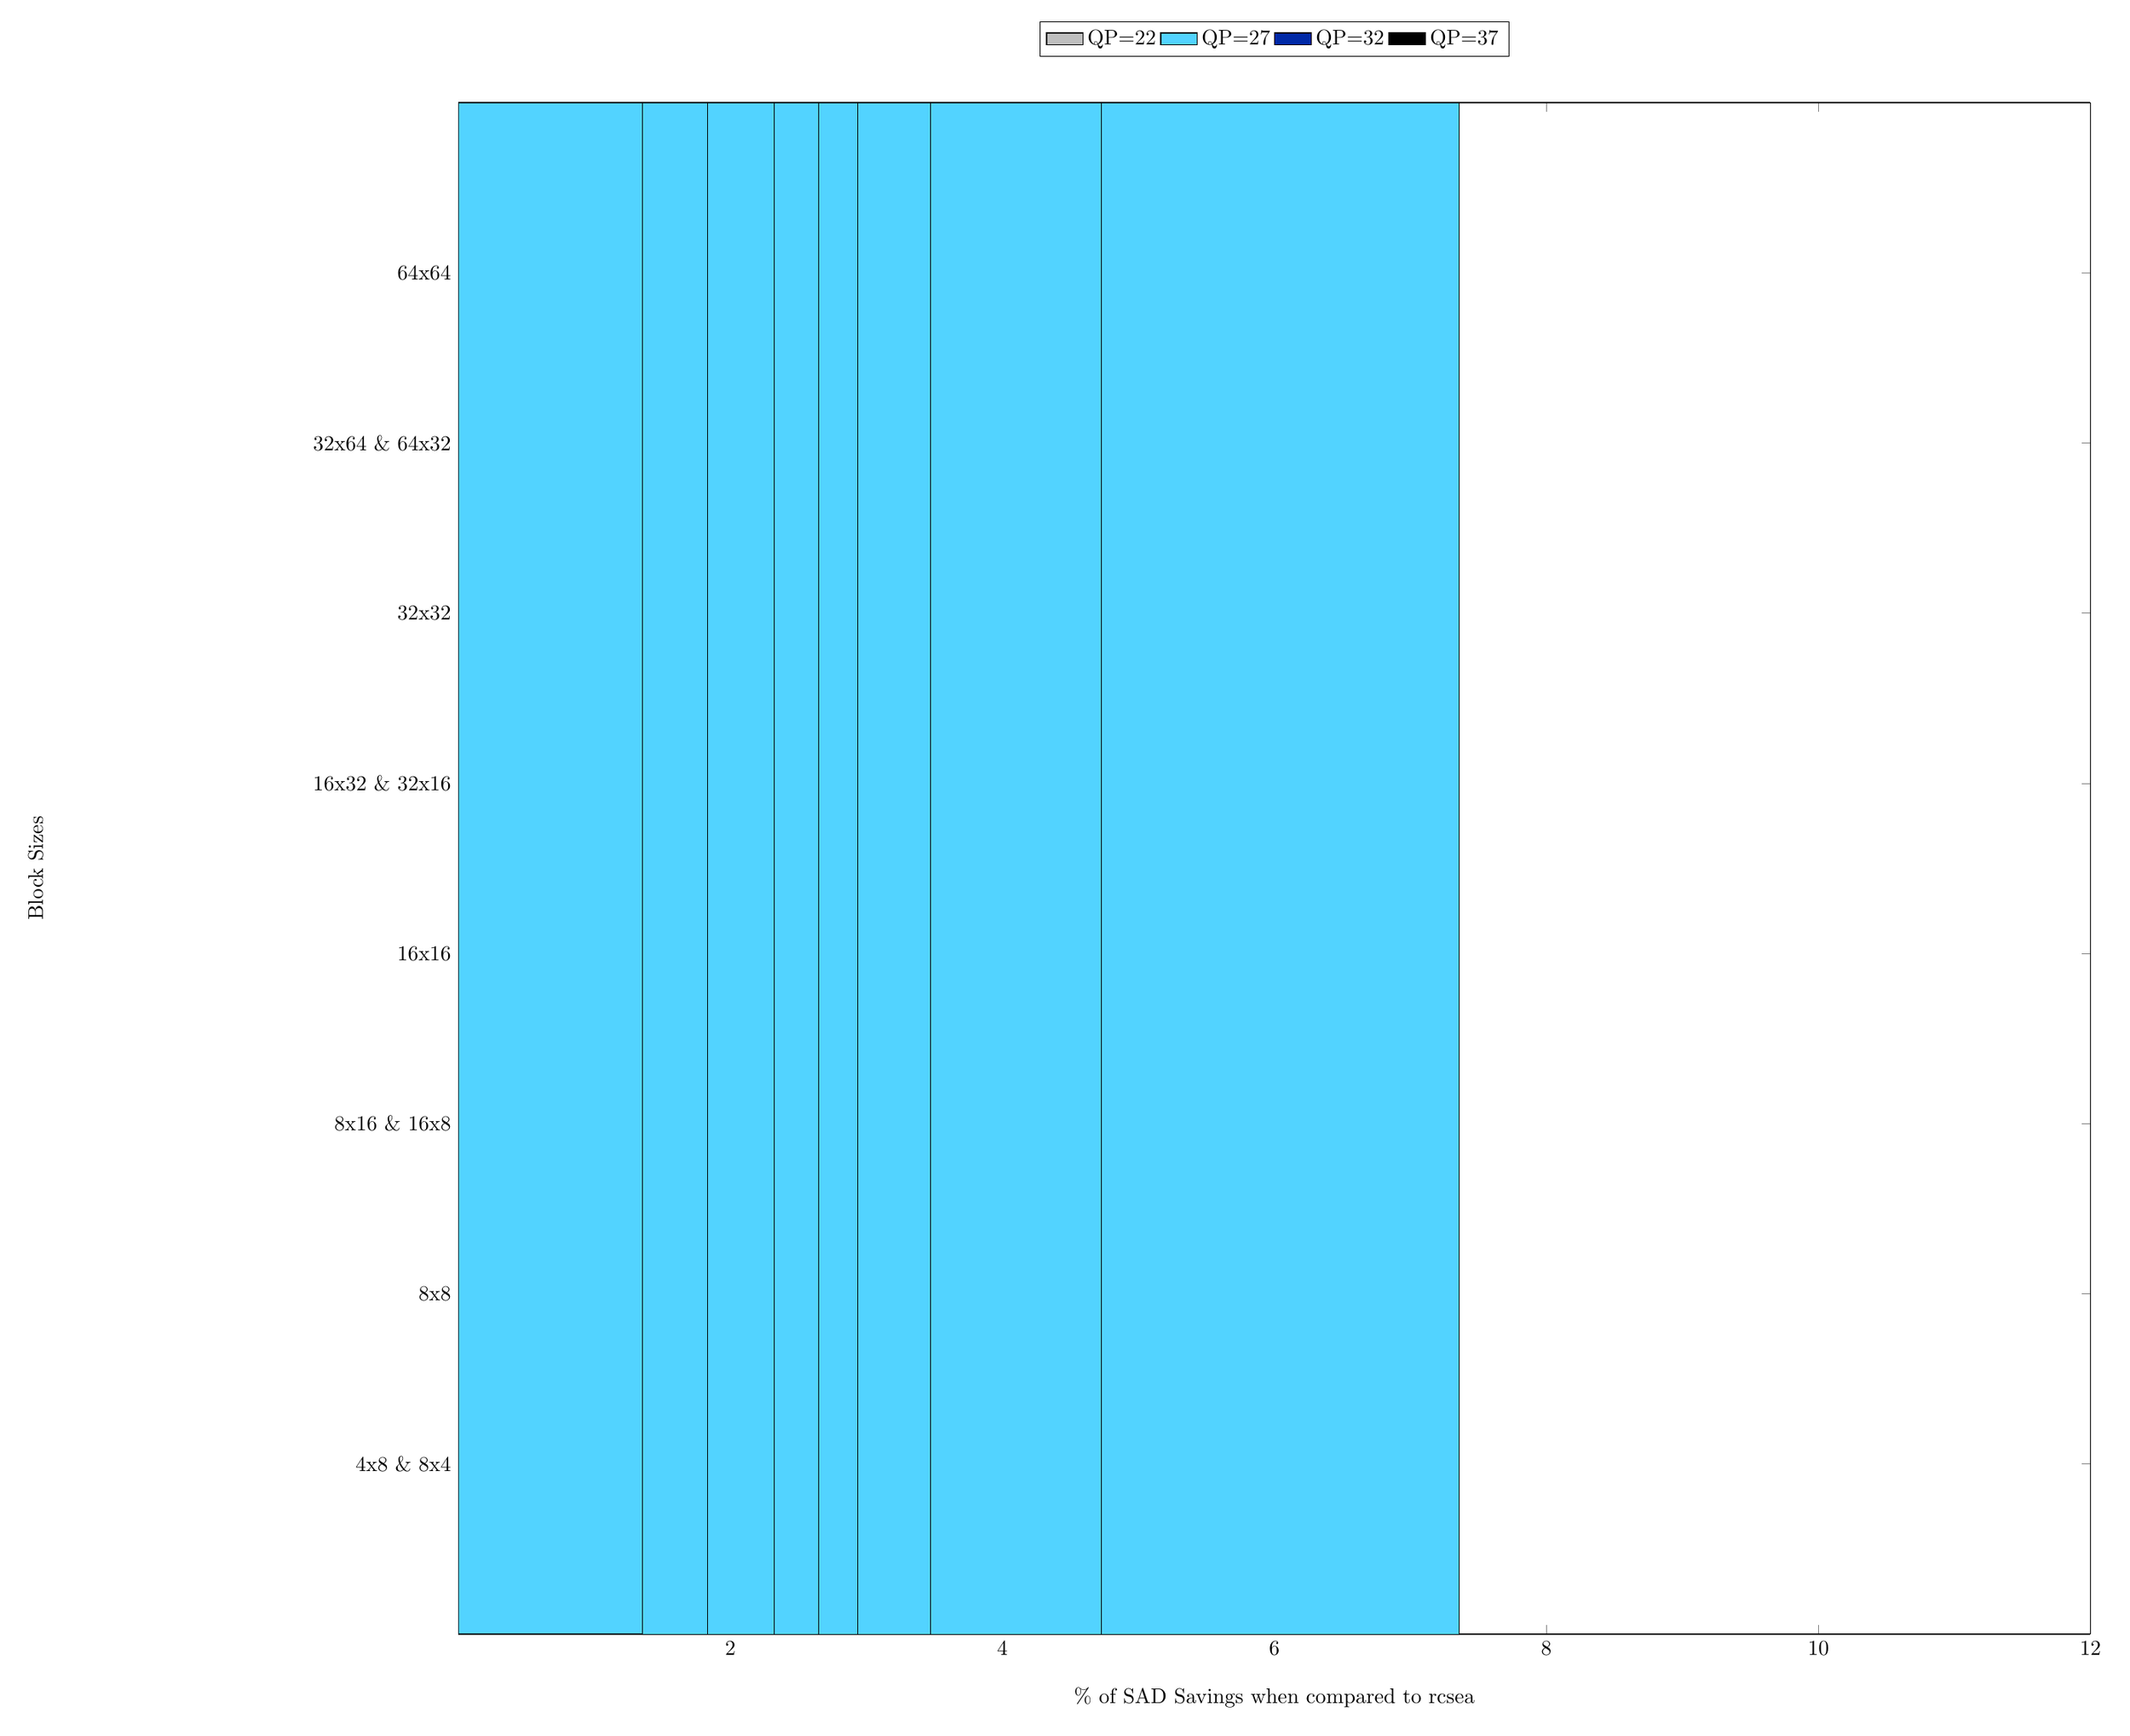
\begin{tikzpicture}

\begin{axis}[%
width=10.65in,
height=10in,
at={(3.464in,1.504in)},
scale only axis,
separate axis lines,
every outer x axis line/.append style={black,},
every x tick label/.append style={font=\color{black}},
xmin=0,
xmax=12,
xtick={2,4,6,8,10,12},
x label style={at={(axis description cs:0.5,-0.03)},anchor=north},
xlabel={\% of SAD Savings when compared to \gls{rcsea}},
every outer y axis line/.append style={black},
every y tick label/.append style={font=\color{black}},
ymin=0,
ymax=9,
ytick={1,2,3,4,5,6,7,8},
yticklabels={{4x8 \& 8x4},{8x8},{8x16 \& 16x8},{16x16},{16x32 \& 32x16},{32x32},{32x64 \& 64x32},{64x64}},
ylabel={Block Sizes},
y label style={at={(axis description cs:-0.25,.5)},anchor=south},
axis background/.style={fill=white},
legend style={at={(0.5,1.03)},anchor=south,legend columns=4,legend cell align=left,align=left,draw=black}
]
\addplot[xbar,bar width=16,bar shift=-18,draw=black,fill=lightgray,area legend] plot table[row sep=crcr] {%
6.2025	1\\
4.2425	2\\
3.455	3\\
3.1	4\\
2.82	5\\
2.4775	6\\
1.9475	7\\
1.4225	8\\
};
\addlegendentry{QP=22};

\addplot [color=black,solid,forget plot]
  table[row sep=crcr]{%
0	0\\
0	9\\
};
\addplot[xbar,bar width=16,bar shift=0,draw=black,fill=mycolor1,area legend] plot table[row sep=crcr] {%
7.3575	1\\
4.725	2\\
3.4725	3\\
2.935	4\\
2.6475	5\\
2.3225	6\\
1.83	7\\
1.355	8\\
};
\addlegendentry{QP=27};

\addplot[xbar,bar width=16,bar shift=18,draw=black,fill=mycolor2,area legend] plot table[row sep=crcr] {%
8.6175	1\\
5.4325	2\\
3.7325	3\\
2.915	4\\
2.58	5\\
2.235	6\\
1.7875	7\\
1.275	8\\
};
\addlegendentry{QP=32};

\addplot[xbar,bar width=16,bar shift=36,draw=black,fill=black,area legend] plot table[row sep=crcr] {%
10.075	1\\
5.935	2\\
3.8325	3\\
2.77	4\\
2.355	5\\
2.0375	6\\
1.6375	7\\
1.215	8\\
};
\addlegendentry{QP=37};

\end{axis}
\end{tikzpicture}%